%----------------------------------------------------------------------------------------
%	PACKAGES AND OTHER DOCUMENT CONFIGURATIONS
%----------------------------------------------------------------------------------------

\documentclass[paper=a4, fontsize=11pt]{scrartcl} % A4 paper and 11pt font size

\usepackage{pgfplots}
\pgfplotsset{compat=1.12}
\usepackage{enumerate}
\usepackage[T1]{fontenc} % Use 8-bit encoding that has 256 glyphs
\usepackage{fourier} % Use the Adobe Utopia font for the document - comment this line to return to the LaTeX default
\usepackage[english]{babel} % English language/hyphenation
\usepackage{amsmath,amsfonts,amsthm} % Math packages

\usepackage{sectsty} % Allows customizing section commands
\allsectionsfont{\centering \normalfont\scshape} % Make all sections centered, the default font and small caps

\usepackage{tkz-graph}
%\usepackage{fancyhdr} % Custom headers and footers
%\pagestyle{fancyplain} % Makes all pages in the document conform to the custom headers and footers
%\fancyhead{} % No page header - if you want one, create it in the same way as the footers below
%\fancyfoot[L]{} % Empty left footer
%\fancyfoot[C]{} % Empty center footer
%\fancyfoot[R]{\thepage} % Page numbering for right footer
%\renewcommand{\headrulewidth}{0pt} % Remove header underlines
%\renewcommand{\footrulewidth}{0pt} % Remove footer underlines
%\setlength{\headheight}{13.6pt} % Customize the height of the header

\numberwithin{equation}{section} % Number equations within sections (i.e. 1.1, 1.2, 2.1, 2.2 instead of 1, 2, 3, 4)
\numberwithin{figure}{section} % Number figures within sections (i.e. 1.1, 1.2, 2.1, 2.2 instead of 1, 2, 3, 4)
\numberwithin{table}{section} % Number tables within sections (i.e. 1.1, 1.2, 2.1, 2.2 instead of 1, 2, 3, 4)

\setlength\parindent{0pt} % Removes all indentation from paragraphs - comment this line for an assignment with lots of text

\newtheorem*{lemma}{Lemma}

%----------------------------------------------------------------------------------------
%	TITLE SECTION
%----------------------------------------------------------------------------------------

%\newcommand{\horrule}[1]{\rule{\linewidth}{#1}} % Create horizontal rule command with 1 argument of height

\title{	
\normalfont \normalsize 
%\horrule{2pt} \\[0.5cm]
\huge Natural Language Processing - Assignment 1 \\ % The assignment title
%\horrule{2pt} \\[0.5cm]
}

\author{
Oran Avraham \texttt{(ID. 203539598)} \quad
Amit Shaked \texttt{(ID. 203119417)}
} % Your name

\date{}

\begin{document}

\maketitle % Print the title

\section{Perplexity vs. $\lambda$-values in Lidstone's smoothing}

\subsection*{N=2}

\begin{center}

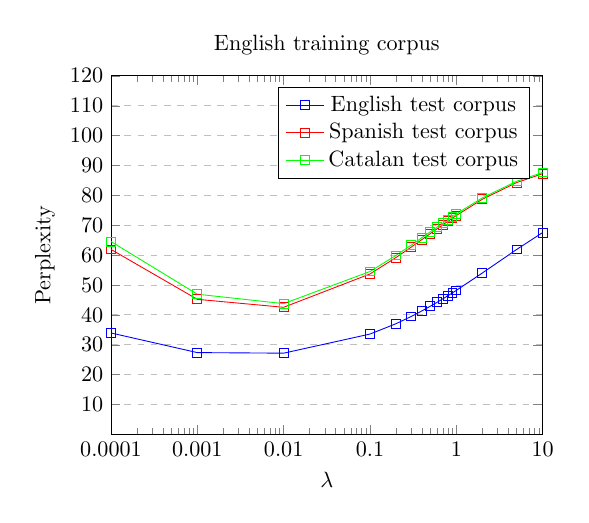
\begin{tikzpicture}[scale=.8]
\begin{semilogxaxis}[
	  log ticks with fixed point,
    title={English training corpus},
    xlabel={$\lambda$},
    ylabel={Perplexity},
    xmin=.0001, xmax=10,
    ymin=0, ymax=120,
    xtick={.0001,.001,.01,.1,1,10},
    ytick={10,20,30,40,50,60,70,80,90,100,110,120},
    legend pos=north east,
    ymajorgrids=true,
    grid style=dashed,
]
 
\addplot[
    color=blue,
    mark=square,
    ]
    coordinates {
(0.00010000,33.9709175258568834)
(0.00100000,27.4005511876346759)
(0.01000000,27.2097439275709441)
(0.10000000,33.5985835905475838)
(0.20000000,37.0677718009028538)
(0.30000000,39.4788092430601907)
(0.40000000,41.3613865129498492)
(0.50000000,42.9165817619826200)
(0.60000000,44.2456519106959192)
(0.70000000,45.4077856958292116)
(0.80000000,46.4409786021626516)
(0.90000000,47.3712514318499558)
(1.00000000,48.2172914439390325)
(2.00000000,54.0290851758192403)
(5.00000000,61.9127302723112507)
(10.00000000,67.5768854086005319)
    };

\addplot[
    color=red,
    mark=square,
    ]
    coordinates {
(0.00010000,61.9293643231486683)
(0.00100000,45.2245332736110939)
(0.01000000,42.5574836721390923)
(0.10000000,53.7101111897372050)
(0.20000000,59.1994413233687524)
(0.30000000,62.6870612303354662)
(0.40000000,65.2315816540894531)
(0.50000000,67.2198384375658122)
(0.60000000,68.8398966326601141)
(0.70000000,70.1982373568702940)
(0.80000000,71.3612447700040917)
(0.90000000,72.3731654469400070)
(1.00000000,73.2649806428615875)
(2.00000000,78.6932003618633900)
(5.00000000,84.2990350925301755)
(10.00000000,87.2566046186265964)
    };

\addplot[
    color=green,
    mark=square,
    ]
    coordinates {
(0.00010000,64.5575648340690549)
(0.00100000,46.9384465764989187)
(0.01000000,43.7812853518558356)
(0.10000000,54.5361862645400990)
(0.20000000,59.9229150217624067)
(0.30000000,63.3570577046293764)
(0.40000000,65.8667623724476385)
(0.50000000,67.8298274646582655)
(0.60000000,69.4304791565654824)
(0.70000000,70.7732314016364938)
(0.80000000,71.9233347272253241)
(0.90000000,72.9243274319720314)
(1.00000000,73.8067212681013416)
(2.00000000,79.1807565363579045)
(5.00000000,84.7333102332676589)
(10.00000000,87.6636747088140567)
    };
    \legend{English test corpus,Spanish test corpus,Catalan test corpus}
 
\end{semilogxaxis}
\end{tikzpicture}
\qquad
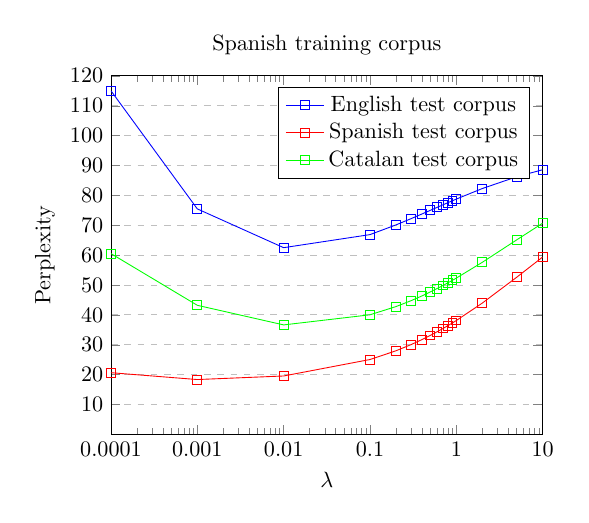
\begin{tikzpicture}[scale=.8]
\begin{semilogxaxis}[
	  log ticks with fixed point,
    title={Spanish training corpus},
    xlabel={$\lambda$},
    ylabel={Perplexity},
    xmin=.0001, xmax=10,
    ymin=0, ymax=120,
    xtick={.0001,.001,.01,.1,1,10},
    ytick={10,20,30,40,50,60,70,80,90,100,110,120},
    legend pos=north east,
    ymajorgrids=true,
    grid style=dashed,
]
 
\addplot[
    color=blue,
    mark=square,
    ]
    coordinates {
(0.00010000,115.0053619565369729)
(0.00100000,75.4853887104112289)
(0.01000000,62.5052614797095600)
(0.10000000,66.8762493662645312)
(0.20000000,70.1252654457947102)
(0.30000000,72.2317168551112729)
(0.40000000,73.7820928246359955)
(0.50000000,75.0017082979238410)
(0.60000000,76.0016187563071526)
(0.70000000,76.8450289737452295)
(0.80000000,77.5714297999730178)
(0.90000000,78.2071695995993821)
(1.00000000,78.7707074594325150)
(2.00000000,82.2934524436399784)
(5.00000000,86.2373777057487416)
(10.00000000,88.5788224852972093)
    };

\addplot[
    color=red,
    mark=square,
    ]
    coordinates {
		(0.00010000,20.6760031479876538)
(0.00100000,18.3840827716670603)
(0.01000000,19.5767372417079635)
(0.10000000,25.0854466667628841)
(0.20000000,28.0077074037100573)
(0.30000000,30.0929036594315171)
(0.40000000,31.7584906104060885)
(0.50000000,33.1611175396782230)
(0.60000000,34.3798112240092379)
(0.70000000,35.4610346149883569)
(0.80000000,36.4348314732418146)
(0.90000000,37.3219375810710758)
(1.00000000,38.1373623781581585)
(2.00000000,43.9724864478504571)
(5.00000000,52.6044758717082743)
(10.00000000,59.3879363348696714)
    };

\addplot[
    color=green,
    mark=square,
    ]
    coordinates {
    (0.00010000,60.5286457523718013)
(0.00100000,43.2242857890149210)
(0.01000000,36.6650279026207997)
(0.10000000,40.0463942016478853)
(0.20000000,42.7977610985461681)
(0.30000000,44.7850729495982378)
(0.40000000,46.3679430611565309)
(0.50000000,47.6938928358624352)
(0.60000000,48.8395240144913316)
(0.70000000,49.8504318750986641)
(0.80000000,50.7562635173611127)
(0.90000000,51.5775269152549143)
(1.00000000,52.3290730155653563)
(2.00000000,57.6114754158890179)
(5.00000000,65.1107296243359599)
(10.00000000,70.7124119486652205)
    };
    \legend{English test corpus,Spanish test corpus,Catalan test corpus}
 
\end{semilogxaxis}
\end{tikzpicture}

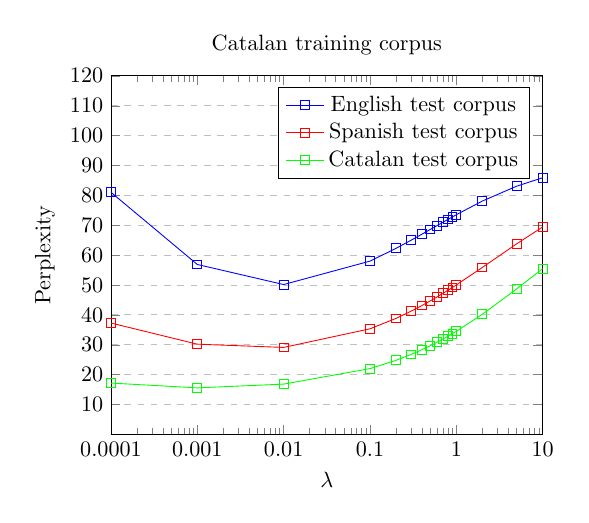
\begin{tikzpicture}[scale=.8]
\begin{semilogxaxis}[
	  log ticks with fixed point,
    title={Catalan training corpus},
    xlabel={$\lambda$},
    ylabel={Perplexity},
    xmin=.0001, xmax=10,
    ymin=0, ymax=120,
    xtick={.0001,.001,.01,.1,1,10},
    ytick={10,20,30,40,50,60,70,80,90,100,110,120},
    legend pos=north east,
    ymajorgrids=true,
    grid style=dashed,
]
 
\addplot[
    color=blue,
    mark=square,
    ]
    coordinates {
    (0.00010000,81.0364047755355870)
(0.00100000,56.8886418281901101)
(0.01000000,50.1662482730151353)
(0.10000000,58.0033848104038228)
(0.20000000,62.2733261742239890)
(0.30000000,65.0125940224562129)
(0.40000000,67.0276174394913511)
(0.50000000,68.6144452022617486)
(0.60000000,69.9169402688004453)
(0.70000000,71.0165552173472747)
(0.80000000,71.9641155871098874)
(0.90000000,72.7935537758674940)
(1.00000000,73.5286816446798355)
(2.00000000,78.1038675737968617)
(5.00000000,83.0883677773916105)
(10.00000000,85.9021779016435545)
    };

\addplot[
    color=red,
    mark=square,
    ]
    coordinates {
    (0.00010000,37.2923115076113945)
(0.00100000,30.2193378967271187)
(0.01000000,29.1309249874060079)
(0.10000000,35.3588271770579823)
(0.20000000,38.8451628287614241)
(0.30000000,41.2653338053674332)
(0.40000000,43.1547831949269067)
(0.50000000,44.7160924137469280)
(0.60000000,46.0509041114217936)
(0.70000000,47.2184977677255304)
(0.80000000,48.2568817992484540)
(0.90000000,49.1920736374679635)
(1.00000000,50.0427579461929355)
(2.00000000,55.8876277313358969)
(5.00000000,63.7974405749786939)
(10.00000000,69.4387859495200814)
    };

\addplot[
    color=green,
    mark=square,
    ]
    coordinates {
    (0.00010000,17.2084235331928639)
(0.00100000,15.6006642684765620)
(0.01000000,16.8531838906264646)
(0.10000000,22.0439732506697013)
(0.20000000,24.8093680467999462)
(0.30000000,26.7930409864643089)
(0.40000000,28.3837506955428900)
(0.50000000,29.7274825109718961)
(0.60000000,30.8980143297787393)
(0.70000000,31.9388042815704694)
(0.80000000,32.8780032012281040)
(0.90000000,33.7350726162849952)
(1.00000000,34.5241212835404525)
(2.00000000,40.2043805187960501)
(5.00000000,48.7166922836574088)
(10.00000000,55.5054185149308594)
    };
    \legend{English test corpus,Spanish test corpus,Catalan test corpus}
 
\end{semilogxaxis}
\end{tikzpicture}

\end{center}

\newpage

\subsection*{N=3}

\begin{center}

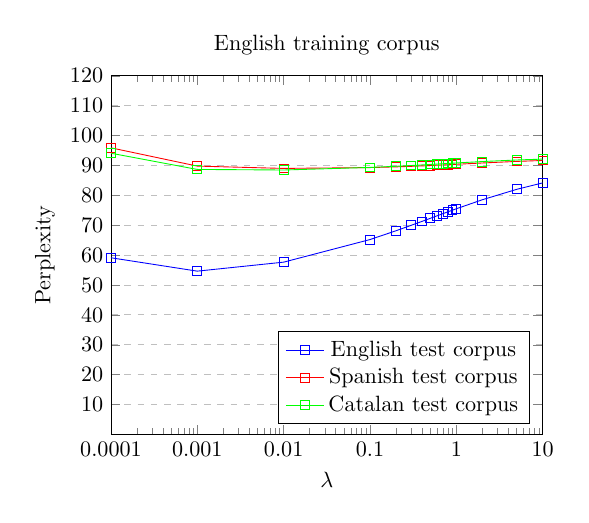
\begin{tikzpicture}[scale=.8]
\begin{semilogxaxis}[
	  log ticks with fixed point,
    title={English training corpus},
    xlabel={$\lambda$},
    ylabel={Perplexity},
    xmin=.0001, xmax=10,
    ymin=0, ymax=120,
    xtick={.0001,.001,.01,.1,1,10},
    ytick={10,20,30,40,50,60,70,80,90,100,110,120},
    legend pos=south east,
    ymajorgrids=true,
    grid style=dashed,
]
 
\addplot[
    color=blue,
    mark=square,
    ]
    coordinates {
(0.00010000,59.1283089317215982)
(0.00100000,54.6517234805657637)
(0.01000000,57.6610332070268115)
(0.10000000,65.2217161334261419)
(0.20000000,68.1635906438678205)
(0.30000000,69.9831803813590625)
(0.40000000,71.3026962861484179)
(0.50000000,72.3347625873169022)
(0.60000000,73.1792631974425802)
(0.70000000,73.8915354220917777)
(0.80000000,74.5055680064687351)
(0.90000000,75.0437767587365698)
(1.00000000,75.5217382188793209)
(2.00000000,78.5401805376036037)
(5.00000000,82.0240976713278229)
(10.00000000,84.1827238467045902)
    };

\addplot[
    color=red,
    mark=square,
    ]
    coordinates {
(0.00010000,95.9125002627099690)
(0.00100000,89.7961286097155948)
(0.01000000,89.0237350415562219)
(0.10000000,89.3062299111504103)
(0.20000000,89.5391996101755296)
(0.30000000,89.7177723781035326)
(0.40000000,89.8632630391371379)
(0.50000000,89.9858010250467970)
(0.60000000,90.0913250052520880)
(0.70000000,90.1836990724573582)
(0.80000000,90.2656028562934125)
(0.90000000,90.3389784351551555)
(1.00000000,90.4052806002390952)
(2.00000000,90.8430598534996392)
(5.00000000,91.3664112136055735)
(10.00000000,91.6813502239128297)
    };

\addplot[
    color=green,
    mark=square,
    ]
    coordinates {
(0.00010000,94.1046507794276152)
(0.00100000,88.6815928254827384)
(0.01000000,88.4936992000500453)
(0.10000000,89.3522510341229435)
(0.20000000,89.7382678865458701)
(0.30000000,89.9955260989669483)
(0.40000000,90.1904259540010429)
(0.50000000,90.3470560356094694)
(0.60000000,90.4774541960382379)
(0.70000000,90.5886622878672512)
(0.80000000,90.6852071296326017)
(0.90000000,90.7701885777525206)
(1.00000000,90.8458283478004063)
(2.00000000,91.3212440525163913)
(5.00000000,91.8434343417199130)
(10.00000000,92.1383844537980821)
    };
    \legend{English test corpus,Spanish test corpus,Catalan test corpus}
 
\end{semilogxaxis}
\end{tikzpicture}
\qquad
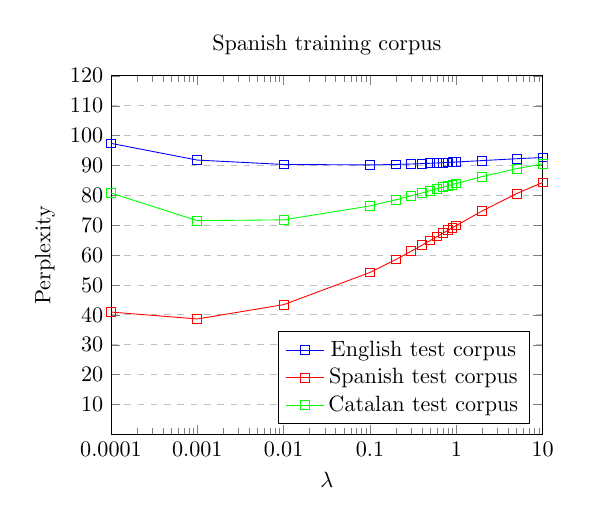
\begin{tikzpicture}[scale=.8]
\begin{semilogxaxis}[
	  log ticks with fixed point,
    title={Spanish training corpus},
    xlabel={$\lambda$},
    ylabel={Perplexity},
    xmin=.0001, xmax=10,
    ymin=0, ymax=120,
    xtick={.0001,.001,.01,.1,1,10},
    ytick={10,20,30,40,50,60,70,80,90,100,110,120},
    legend pos=south east,
    ymajorgrids=true,
    grid style=dashed,
]
 
\addplot[
    color=blue,
    mark=square,
    ]
    coordinates {
(0.00010000,97.4011888994087229)
(0.00100000,91.8113326669431586)
(0.01000000,90.3481014923758181)
(0.10000000,90.1910296056551601)
(0.20000000,90.3474557963722447)
(0.30000000,90.4975810808364827)
(0.40000000,90.6305084994941978)
(0.50000000,90.7476055741140328)
(0.60000000,90.8514097703866099)
(0.70000000,90.9441960143815038)
(0.80000000,91.0278085551387193)
(0.90000000,91.1037126289304666)
(1.00000000,91.1730737726991123)
(2.00000000,91.6488940732536150)
(5.00000000,92.2646209199521508)
(10.00000000,92.6712659443569038)
    };

\addplot[
    color=red,
    mark=square,
    ]
    coordinates {
(0.00010000,40.9639438998515004)
(0.00100000,38.6584153753228321)
(0.01000000,43.4415292344909076)
(0.10000000,54.2127005765265864)
(0.20000000,58.5692680167594588)
(0.30000000,61.3160844954069475)
(0.40000000,63.3332253349566443)
(0.50000000,64.9260564481858182)
(0.60000000,66.2395547276860839)
(0.70000000,67.3546940599671444)
(0.80000000,68.3215397850509021)
(0.90000000,69.1732970830234564)
(1.00000000,69.9331545756946582)
(2.00000000,74.8108793989151906)
(5.00000000,80.6206980976027552)
(10.00000000,84.3101043065777560)
    };

\addplot[
    color=green,
    mark=square,
    ]
    coordinates {
(0.00010000,80.7829345245770583)
(0.00100000,71.5528274889652209)
(0.01000000,71.8107081026033853)
(0.10000000,76.4706463647400909)
(0.20000000,78.5317674948841216)
(0.30000000,79.8503846726142399)
(0.40000000,80.8228044752091819)
(0.50000000,81.5911509778608774)
(0.60000000,82.2241320243881120)
(0.70000000,82.7605660652243529)
(0.80000000,83.2246406959750828)
(0.90000000,83.6324846758130462)
(1.00000000,83.9954043529956351)
(2.00000000,86.2967780687710331)
(5.00000000,88.9439727679360601)
(10.00000000,90.5526988538777005)
    };
    \legend{English test corpus,Spanish test corpus,Catalan test corpus}
 
\end{semilogxaxis}
\end{tikzpicture}

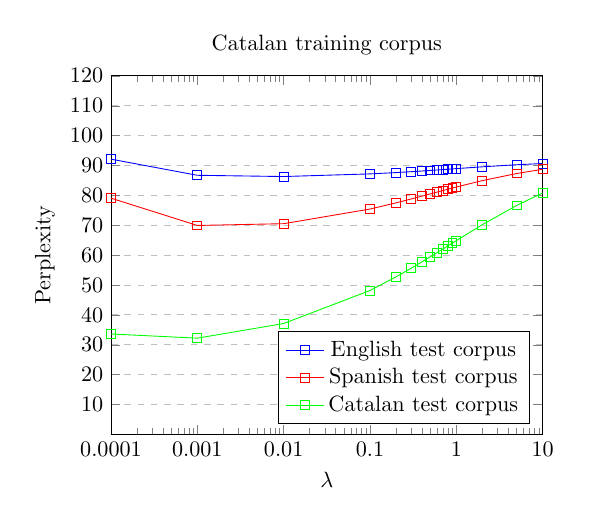
\begin{tikzpicture}[scale=.8]
\begin{semilogxaxis}[
	  log ticks with fixed point,
    title={Catalan training corpus},
    xlabel={$\lambda$},
    ylabel={Perplexity},
    xmin=.0001, xmax=10,
    ymin=0, ymax=120,
    xtick={.0001,.001,.01,.1,1,10},
    ytick={10,20,30,40,50,60,70,80,90,100,110,120},
    legend pos=south east,
    ymajorgrids=true,
    grid style=dashed,
]
 
\addplot[
    color=blue,
    mark=square,
    ]
    coordinates {
(0.00010000,92.1240701265360258)
(0.00100000,86.7242459209968075)
(0.01000000,86.3077754914684476)
(0.10000000,87.1903408517123353)
(0.20000000,87.6277188157458937)
(0.30000000,87.9276816442450837)
(0.40000000,88.1586557165922358)
(0.50000000,88.3464086947996634)
(0.60000000,88.5041310168937230)
(0.70000000,88.6396664007994559)
(0.80000000,88.7581167123006622)
(0.90000000,88.8630065781164831)
(1.00000000,88.9568797914650702)
(2.00000000,89.5594574975564655)
(5.00000000,90.2524660257874984)
(10.00000000,90.6602507930754911)
    };

\addplot[
    color=red,
    mark=square,
    ]
    coordinates {
(0.00010000,79.0766895724054990)
(0.00100000,69.9389145669934322)
(0.01000000,70.5322378695885419)
(0.10000000,75.4258936041369736)
(0.20000000,77.4968810265583983)
(0.30000000,78.8019379999643519)
(0.40000000,79.7549068495853675)
(0.50000000,80.5020333991339641)
(0.60000000,81.1134573261355740)
(0.70000000,81.6285916757146168)
(0.80000000,82.0718907384428178)
(0.90000000,82.4596023787350560)
(1.00000000,82.8030795142188367)
(2.00000000,84.9447909416295630)
(5.00000000,87.3226009360844841)
(10.00000000,88.7221523172377431)
    };

\addplot[
    color=green,
    mark=square,
    ]
    coordinates {
(0.00010000,33.6300430098770633)
(0.00100000,32.2281295519186131)
(0.01000000,37.1268291594521500)
(0.10000000,48.1674725711669325)
(0.20000000,52.7301967956830921)
(0.30000000,55.6316770632262276)
(0.40000000,57.7746847350702524)
(0.50000000,59.4744940549447492)
(0.60000000,60.8814196644865007)
(0.70000000,62.0796932293630093)
(0.80000000,63.1215385142198571)
(0.90000000,64.0416763035989050)
(1.00000000,64.8644065435427990)
(2.00000000,70.1905597353149346)
(5.00000000,76.6487554621150196)
(10.00000000,80.8246520215136002)
    };
    \legend{English test corpus,Spanish test corpus,Catalan test corpus}
 
\end{semilogxaxis}
\end{tikzpicture}

\end{center}

\newpage

\subsection*{N=4}

\begin{center}

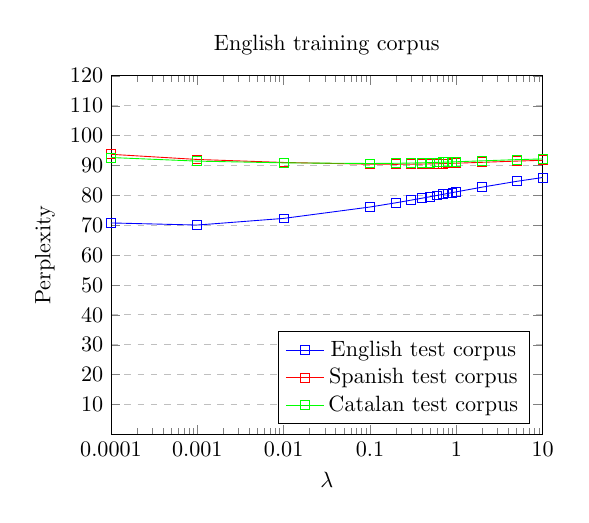
\begin{tikzpicture}[scale=.8]
\begin{semilogxaxis}[
	  log ticks with fixed point,
    title={English training corpus},
    xlabel={$\lambda$},
    ylabel={Perplexity},
    xmin=.0001, xmax=10,
    ymin=0, ymax=120,
    xtick={.0001,.001,.01,.1,1,10},
    ytick={10,20,30,40,50,60,70,80,90,100,110,120},
    legend pos=south east,
    ymajorgrids=true,
    grid style=dashed,
]
 
\addplot[
    color=blue,
    mark=square,
    ]
    coordinates {
(0.00010000,70.7838359216829787)
(0.00100000,70.0739347789917986)
(0.01000000,72.2985689054383442)
(0.10000000,76.1112575719986637)
(0.20000000,77.5275960540965059)
(0.30000000,78.4110212760483734)
(0.40000000,79.0585485541039645)
(0.50000000,79.5700561716805197)
(0.60000000,79.9923144645533739)
(0.70000000,80.3512721271907679)
(0.80000000,80.6629202278716662)
(0.90000000,80.9378480836673617)
(1.00000000,81.1834458751035442)
(2.00000000,82.7700533251326362)
(5.00000000,84.7015648800841063)
(10.00000000,85.9794225151844529)
    };

\addplot[
    color=red,
    mark=square,
    ]
    coordinates {
(0.00010000,93.7409203556402417)
(0.00100000,92.0182444977026819)
(0.01000000,91.0212602048615054)
(0.10000000,90.4230208013376000)
(0.20000000,90.3934129128273582)
(0.30000000,90.4286476652002165)
(0.40000000,90.4789841584193084)
(0.50000000,90.5321812430743336)
(0.60000000,90.5842677606294018)
(0.70000000,90.6338749255175742)
(0.80000000,90.6805991298397771)
(0.90000000,90.7244231639468239)
(1.00000000,90.7654856315493390)
(2.00000000,91.0655139391036812)
(5.00000000,91.4748648613262674)
(10.00000000,91.7415285911387741)
    };

\addplot[
    color=green,
    mark=square,
    ]
    coordinates {
(0.00010000,92.6689697631915124)
(0.00100000,91.4602383881187251)
(0.01000000,90.8863995755205849)
(0.10000000,90.6722033006077055)
(0.20000000,90.7400203907206446)
(0.30000000,90.8239329562637181)
(0.40000000,90.9040457134869371)
(0.50000000,90.9772514576050497)
(0.60000000,91.0435333854303650)
(0.70000000,91.1035665891842683)
(0.80000000,91.1581269891126027)
(0.90000000,91.2079317376320375)
(1.00000000,91.2536028044347347)
(2.00000000,91.5671506411171237)
(5.00000000,91.9590873678890546)
(10.00000000,92.2008818487639275)
    };
    \legend{English test corpus,Spanish test corpus,Catalan test corpus}
 
\end{semilogxaxis}
\end{tikzpicture}
\qquad
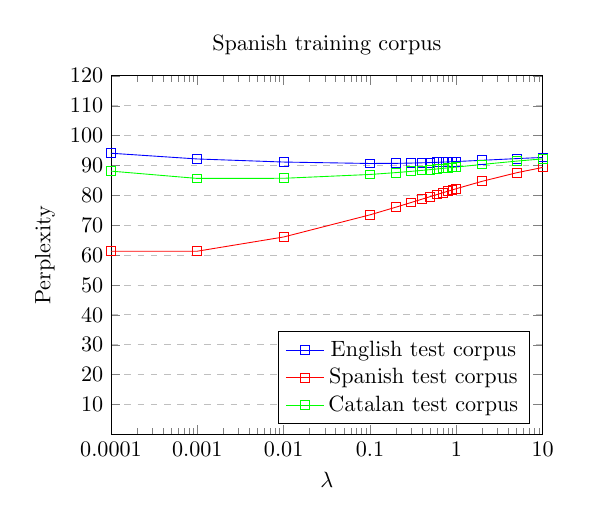
\begin{tikzpicture}[scale=.8]
\begin{semilogxaxis}[
	  log ticks with fixed point,
    title={Spanish training corpus},
    xlabel={$\lambda$},
    ylabel={Perplexity},
    xmin=.0001, xmax=10,
    ymin=0, ymax=120,
    xtick={.0001,.001,.01,.1,1,10},
    ytick={10,20,30,40,50,60,70,80,90,100,110,120},
    legend pos=south east,
    ymajorgrids=true,
    grid style=dashed,
]
 
\addplot[
    color=blue,
    mark=square,
    ]
    coordinates {
(0.00010000,94.1051565833287640)
(0.00100000,92.1852341309041350)
(0.01000000,91.1555916836022817)
(0.10000000,90.6777474967318682)
(0.20000000,90.7210107822816099)
(0.30000000,90.8084710839428340)
(0.40000000,90.8995597802098700)
(0.50000000,90.9860712626818184)
(0.60000000,91.0662574819790933)
(0.70000000,91.1401164525290994)
(0.80000000,91.2081452693207666)
(0.90000000,91.2709504755167131)
(1.00000000,91.3291193874974283)
(2.00000000,91.7438604909954023)
(5.00000000,92.3094410432263146)
(10.00000000,92.6953563315656197)
    };

\addplot[
    color=red,
    mark=square,
    ]
    coordinates {
(0.00010000,61.3100703532033791)
(0.00100000,61.3271455611933831)
(0.01000000,66.0822404749107619)
(0.10000000,73.4898199543197421)
(0.20000000,76.0658873471014658)
(0.30000000,77.6207495700976722)
(0.40000000,78.7352430220479391)
(0.50000000,79.6008155827436212)
(0.60000000,80.3056674646814628)
(0.70000000,80.8980503038770280)
(0.80000000,81.4073356010243145)
(0.90000000,81.8527626210421602)
(1.00000000,82.2476287177819643)
(2.00000000,84.7291104294536410)
(5.00000000,87.5787107352852132)
(10.00000000,89.3461332722549457)
    };

\addplot[
    color=green,
    mark=square,
    ]
    coordinates {
(0.00010000,88.1229201316707673)
(0.00100000,85.6719540751590216)
(0.01000000,85.7197790593851607)
(0.10000000,86.9979904057530149)
(0.20000000,87.6226302067387905)
(0.30000000,88.0435202415742140)
(0.40000000,88.3651218969876595)
(0.50000000,88.6260518476881032)
(0.60000000,88.8455534578886272)
(0.70000000,89.0348029167840025)
(0.80000000,89.2009340469913781)
(0.90000000,89.3488039177523774)
(1.00000000,89.4818791028892804)
(2.00000000,90.3609707510764792)
(5.00000000,91.4675614587979169)
(10.00000000,92.2160959291668405)
    };
    \legend{English test corpus,Spanish test corpus,Catalan test corpus}
 
\end{semilogxaxis}
\end{tikzpicture}

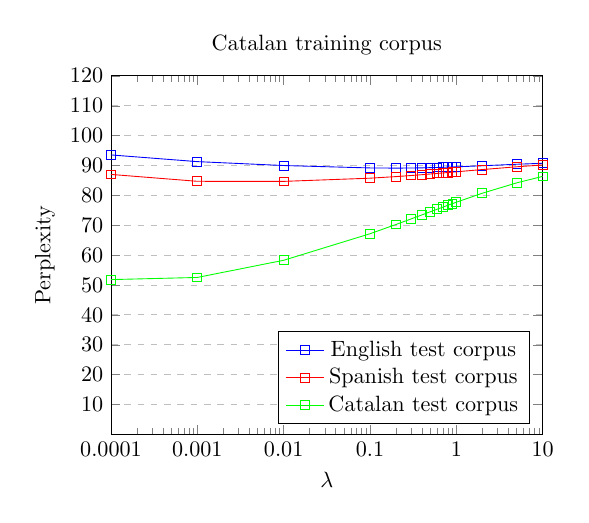
\begin{tikzpicture}[scale=.8]
\begin{semilogxaxis}[
	  log ticks with fixed point,
    title={Catalan training corpus},
    xlabel={$\lambda$},
    ylabel={Perplexity},
    xmin=.0001, xmax=10,
    ymin=0, ymax=120,
    xtick={.0001,.001,.01,.1,1,10},
    ytick={10,20,30,40,50,60,70,80,90,100,110,120},
    legend pos=south east,
    ymajorgrids=true,
    grid style=dashed,
]
 
\addplot[
    color=blue,
    mark=square,
    ]
    coordinates {
(0.00010000,93.5356597887484753)
(0.00100000,91.2953675472633392)
(0.01000000,89.9904532262239485)
(0.10000000,89.1817857495172177)
(0.20000000,89.1281315994347096)
(0.30000000,89.1622677169337408)
(0.40000000,89.2179159825322614)
(0.50000000,89.2786386279231579)
(0.60000000,89.3389844332829881)
(0.70000000,89.3969763822136940)
(0.80000000,89.4519420980331574)
(0.90000000,89.5037442745468184)
(1.00000000,89.5524716136864356)
(2.00000000,89.9129289187149681)
(5.00000000,90.4146778026439506)
(10.00000000,90.7462909859893472)
    };

\addplot[
    color=red,
    mark=square,
    ]
    coordinates {
(0.00010000,87.0130605277985296)
(0.00100000,84.7130529840393081)
(0.01000000,84.6863880013999193)
(0.10000000,85.7540746740866524)
(0.20000000,86.2875977057031776)
(0.30000000,86.6497876759663939)
(0.40000000,86.9274516607664083)
(0.50000000,87.1530142394875611)
(0.60000000,87.3427860385378949)
(0.70000000,87.5063142053992209)
(0.80000000,87.6497309858935694)
(0.90000000,87.7772322391922586)
(1.00000000,87.8918242929521796)
(2.00000000,88.6434976626522655)
(5.00000000,89.5712585312341645)
(10.00000000,90.1864223742098119)
    };

\addplot[
    color=green,
    mark=square,
    ]
    coordinates {
(0.00010000,51.8226074786520314)
(0.00100000,52.5424636600586865)
(0.01000000,58.2870091863047080)
(0.10000000,67.1657819505705618)
(0.20000000,70.2662631977654826)
(0.30000000,72.1383778299454406)
(0.40000000,73.4805756297370607)
(0.50000000,74.5233500242723039)
(0.60000000,75.3728759972319580)
(0.70000000,76.0872099855961608)
(0.80000000,76.7016726637668000)
(0.90000000,77.2393890549036684)
(1.00000000,77.7163359811629562)
(2.00000000,80.7211392303671715)
(5.00000000,84.1925693023529931)
(10.00000000,86.3567220085654270)
    };
    \legend{English test corpus,Spanish test corpus,Catalan test corpus}
 
\end{semilogxaxis}
\end{tikzpicture}

\end{center}

\subsection*{Conclusions}

\begin{itemize}
	\item Larger n-gram means larger perplexity values.
	\item Larger $\lambda$-values might mean smaller perplexity values for very small $\lambda$-values, but for $\lambda \geq 0.01$
		the perplexity increases as $\lambda$ increases (the graph is convex).
	\item As $\lambda$ increases, the difference between condition positive (true language) perplexity and condition negative
		(false language) perplexity decreases (this is more noticeable for two-grams and three-grams). This might be due to the fact
		that larger $\lambda$-values means that the distribution is closer to uniform distribution.
	\item In our case, $\lambda=10^{-3}$ seems to be the value for which the perplexity is minimal for the true test language. However,
	the difference in the perplexity of the true language between $\lambda=10^{-4}$ and $\lambda=10^{-3}$ is negligible, while for false
	languages there is a large difference. Hence, since our purpose is language detection, we chose $\lambda=10^{-4}$.
\end{itemize}

\newpage
\section{Witten-Bell compared to Lidstone's smoothing}

We chose $\lambda=10^{-4}$ for Lidstone's smoothing as explained in previous section.

\subsection*{N=2}

\begin{center}

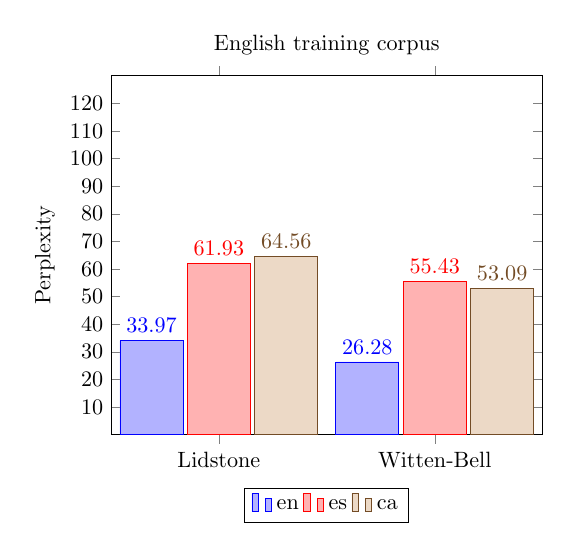
\begin{tikzpicture}[scale=.8]
\begin{axis}[
	title={English training corpus},
	ybar,
	enlarge x limits=0.5,
	legend style={at={(0.5,-0.15)}, anchor=north,legend columns=-1},
	ylabel={Perplexity},
	symbolic x coords={Lidstone,Witten-Bell},
	xtick=data,
	ymin=0, ymax=130,
	ytick={10,20,30,40,50,60,70,80,90,100,110,120},
	bar width=1cm,
	nodes near coords,
]
\addplot coordinates {(Lidstone,33.9709175258568834) (Witten-Bell,26.2813386380639109)};
\addplot coordinates {(Lidstone,61.9293643231486683) (Witten-Bell,55.4296898751559795)};
\addplot coordinates {(Lidstone,64.5575648340690549) (Witten-Bell,53.0874135920790380)};
\legend{en,es,ca}
\end{axis}
\end{tikzpicture}
\qquad
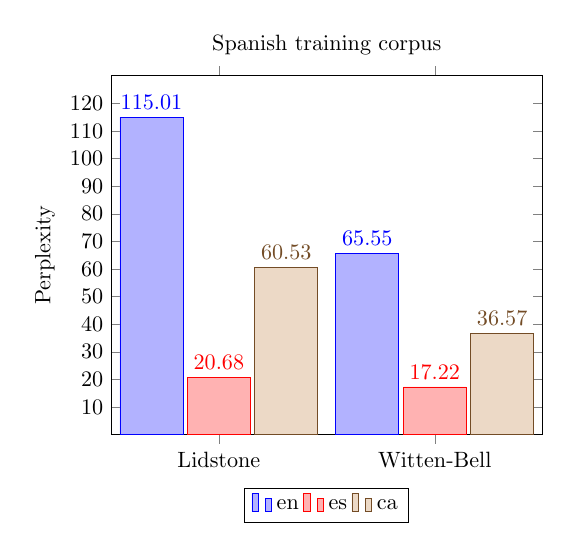
\begin{tikzpicture}[scale=.8]
\begin{axis}[
	title={Spanish training corpus},
	ybar,
	enlarge x limits=0.5,
	legend style={at={(0.5,-0.15)}, anchor=north,legend columns=-1},
	ylabel={Perplexity},
	symbolic x coords={Lidstone,Witten-Bell},
	xtick=data,
	ymin=0, ymax=130,
	ytick={10,20,30,40,50,60,70,80,90,100,110,120},
	bar width=1cm,
	nodes near coords,
]
\addplot coordinates {(Lidstone,115.0053619565369729) (Witten-Bell,65.5467578637442472)};
\addplot coordinates {(Lidstone,20.6760031479876538) (Witten-Bell,17.2177660276275013)};
\addplot coordinates {(Lidstone,60.5286457523718013) (Witten-Bell,36.5671173426087606)};
\legend{en,es,ca}
\end{axis}
\end{tikzpicture}

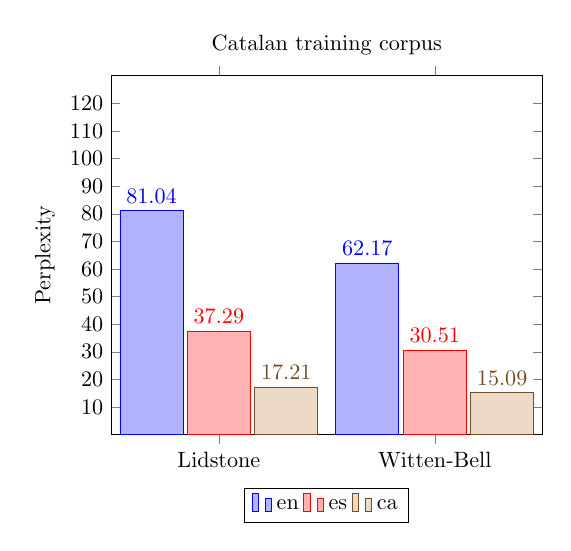
\begin{tikzpicture}[scale=.8]
\begin{axis}[
	title={Catalan training corpus},
	ybar,
	enlarge x limits=0.5,
	legend style={at={(0.5,-0.15)}, anchor=north,legend columns=-1},
	ylabel={Perplexity},
	symbolic x coords={Lidstone,Witten-Bell},
	xtick=data,
	ymin=0, ymax=130,
	ytick={10,20,30,40,50,60,70,80,90,100,110,120},
	bar width=1cm,
	nodes near coords,
]
\addplot coordinates {(Lidstone,81.0364047755355870) (Witten-Bell,62.1660478904621527)};
\addplot coordinates {(Lidstone,37.2923115076113945) (Witten-Bell,30.5072434974184787)};
\addplot coordinates {(Lidstone,17.2084235331928639) (Witten-Bell,15.0877099149183511)};
\legend{en,es,ca}
\end{axis}
\end{tikzpicture}

\end{center}

\newpage
\subsection*{N=3}

\begin{center}

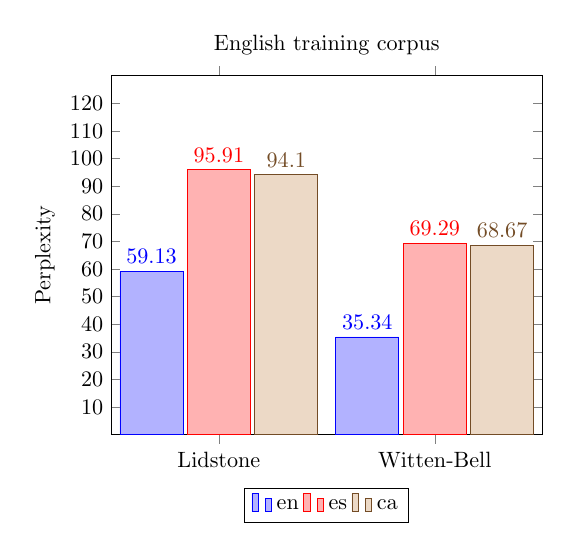
\begin{tikzpicture}[scale=.8]
\begin{axis}[
	title={English training corpus},
	ybar,
	enlarge x limits=0.5,
	legend style={at={(0.5,-0.15)}, anchor=north,legend columns=-1},
	ylabel={Perplexity},
	symbolic x coords={Lidstone,Witten-Bell},
	xtick=data,
	ymin=0, ymax=130,
	ytick={10,20,30,40,50,60,70,80,90,100,110,120},
	bar width=1cm,
	nodes near coords,
]
\addplot coordinates {(Lidstone,59.1283089317215982) (Witten-Bell,35.3392196020463203)};
\addplot coordinates {(Lidstone,95.9125002627099690) (Witten-Bell,69.2914739187706914)};
\addplot coordinates {(Lidstone,94.1046507794276152) (Witten-Bell,68.6735491041301742)};
\legend{en,es,ca}
\end{axis}
\end{tikzpicture}
\qquad
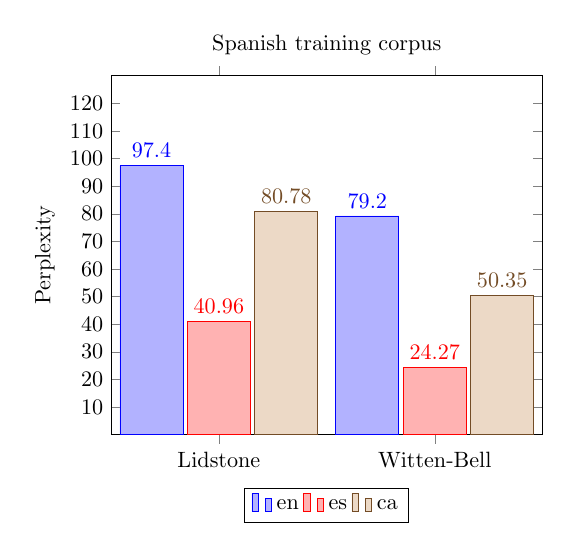
\begin{tikzpicture}[scale=.8]
\begin{axis}[
	title={Spanish training corpus},
	ybar,
	enlarge x limits=0.5,
	legend style={at={(0.5,-0.15)}, anchor=north,legend columns=-1},
	ylabel={Perplexity},
	symbolic x coords={Lidstone,Witten-Bell},
	xtick=data,
	ymin=0, ymax=130,
	ytick={10,20,30,40,50,60,70,80,90,100,110,120},
	bar width=1cm,
	nodes near coords,
]
\addplot coordinates {(Lidstone,97.4011888994087229) (Witten-Bell,79.2032399414232628)};
\addplot coordinates {(Lidstone,40.9639438998515004) (Witten-Bell,24.2690525366963570)};
\addplot coordinates {(Lidstone,80.7829345245770583) (Witten-Bell,50.3545705852040442)};
\legend{en,es,ca}
\end{axis}
\end{tikzpicture}

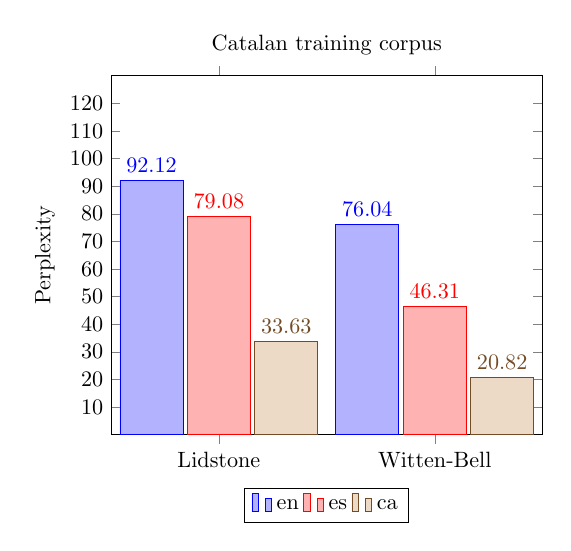
\begin{tikzpicture}[scale=.8]
\begin{axis}[
	title={Catalan training corpus},
	ybar,
	enlarge x limits=0.5,
	legend style={at={(0.5,-0.15)}, anchor=north,legend columns=-1},
	ylabel={Perplexity},
	symbolic x coords={Lidstone,Witten-Bell},
	xtick=data,
	ymin=0, ymax=130,
	ytick={10,20,30,40,50,60,70,80,90,100,110,120},
	bar width=1cm,
	nodes near coords,
]
\addplot coordinates {(Lidstone,92.1240701265360258) (Witten-Bell,76.0432071881298270)};
\addplot coordinates {(Lidstone,79.0766895724054990) (Witten-Bell,46.3116987920521836)};
\addplot coordinates {(Lidstone,33.6300430098770633) (Witten-Bell,20.8166778217064490)};
\legend{en,es,ca}
\end{axis}
\end{tikzpicture}

\end{center}

\newpage
\subsection*{N=4}

\begin{center}

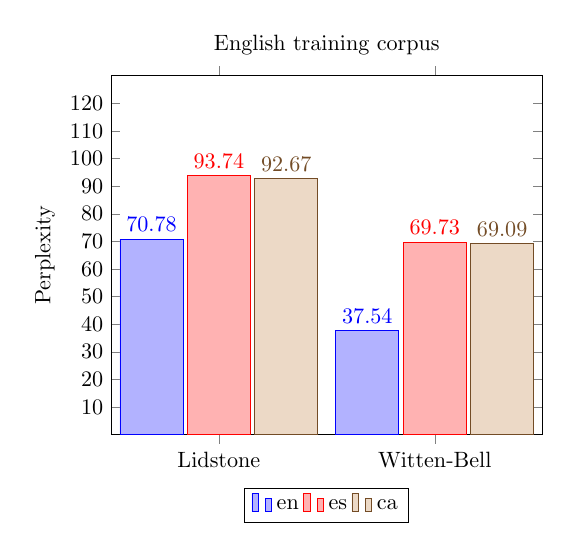
\begin{tikzpicture}[scale=.8]
\begin{axis}[
	title={English training corpus},
	ybar,
	enlarge x limits=0.5,
	legend style={at={(0.5,-0.15)}, anchor=north,legend columns=-1},
	ylabel={Perplexity},
	symbolic x coords={Lidstone,Witten-Bell},
	xtick=data,
	ymin=0, ymax=130,
	ytick={10,20,30,40,50,60,70,80,90,100,110,120},
	bar width=1cm,
	nodes near coords,
]
\addplot coordinates {(Lidstone,70.7838359216829787) (Witten-Bell,37.5384609732930841)};
\addplot coordinates {(Lidstone,93.7409203556402417) (Witten-Bell,69.7335551150016499)};
\addplot coordinates {(Lidstone,92.6689697631915124) (Witten-Bell,69.0850906203342134)};
\legend{en,es,ca}
\end{axis}
\end{tikzpicture}
\qquad
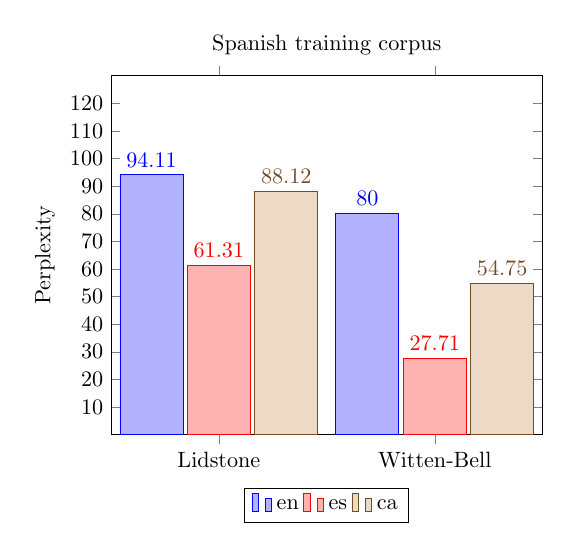
\begin{tikzpicture}[scale=.8]
\begin{axis}[
	title={Spanish training corpus},
	ybar,
	enlarge x limits=0.5,
	legend style={at={(0.5,-0.15)}, anchor=north,legend columns=-1},
	ylabel={Perplexity},
	symbolic x coords={Lidstone,Witten-Bell},
	xtick=data,
	ymin=0, ymax=130,
	ytick={10,20,30,40,50,60,70,80,90,100,110,120},
	bar width=1cm,
	nodes near coords,
]
\addplot coordinates {(Lidstone,94.1051565833287640) (Witten-Bell,79.9952132127366156)};
\addplot coordinates {(Lidstone,61.3100703532033791) (Witten-Bell,27.7121024323646807)};
\addplot coordinates {(Lidstone,88.1229201316707673) (Witten-Bell,54.7508602837030196)};
\legend{en,es,ca}
\end{axis}
\end{tikzpicture}

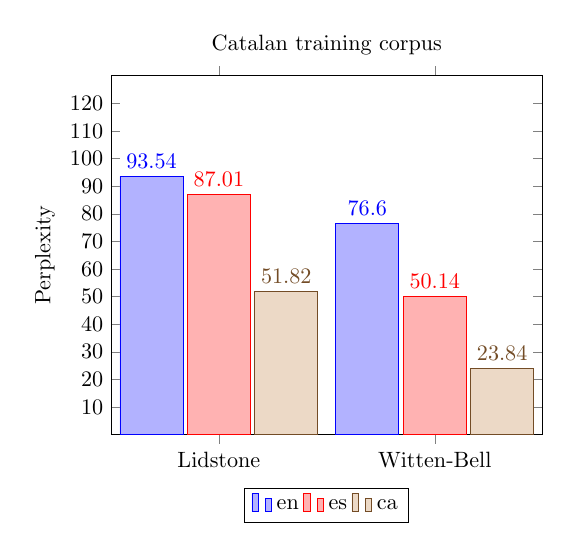
\begin{tikzpicture}[scale=.8]
\begin{axis}[
	title={Catalan training corpus},
	ybar,
	enlarge x limits=0.5,
	legend style={at={(0.5,-0.15)}, anchor=north,legend columns=-1},
	ylabel={Perplexity},
	symbolic x coords={Lidstone,Witten-Bell},
	xtick=data,
	ymin=0, ymax=130,
	ytick={10,20,30,40,50,60,70,80,90,100,110,120},
	bar width=1cm,
	nodes near coords,
]
\addplot coordinates {(Lidstone,93.5356597887484753) (Witten-Bell,76.5965039173272828)};
\addplot coordinates {(Lidstone,87.0130605277985296) (Witten-Bell,50.1368336506490166)};
\addplot coordinates {(Lidstone,51.8226074786520314) (Witten-Bell,23.8370767925576494)};
\legend{en,es,ca}
\end{axis}
\end{tikzpicture}

\end{center}

\subsection*{Conclusions}

\begin{itemize}
	\item Witten-Bell smoothing generally produces lower perplexity values than Lidstone's.
	\item As $n$ increases, the increase in perplexity values in Lidstone's smoothing is much larger than in Witten-Bell smoothing.
	\item For four-grams, Lidstone's smoothing showed large difference in perplexity values between Spanish and Catalan;
		Witten-Bell, however, showed smaller difference. This may be due to the fact that we incorporated interpolation in Witten-Bell, thus
		smaller n-grams probabilities are also considered.
\end{itemize}

\section{Language detection}

In the previous section we've seen that Witten-Bell smoothing produces lower perplexity values than Lidstone's,
thus it models the language better. We would like to find the language model which suits our needs the best.

For two-grams, Spanish and Catalan seem to be too close to one another (when a Spanish corpus was tested against a Catalan model,
there was a 15.42 difference in perplexity).

The results for three-grams and four-grams seemed to be somewhat similar; however, three-grams had lower perplexity values for the real
language. In addition, as we've seen, four-grams is prone to overfitting (it models the training corpus instead of the language). Therefore,
we chose $n=3$ with Witten-Bell smoothing.

We've detected correctly $95\%$ of the sentences: $94\%$ of the English sentences, $96.5\%$ of the Spanish sentences and $95\%$ of the Catalan sentences.

Whenever we failed to identify a Spanish sentence, we identified it as Catalan. The opposite wasn't true (we did identify Catalan sentences as English).

Besides the language model, another option to implement language detection is to use a lexicon - for each language, store a lexicon
of known words in this language; process the test corpus and find which lexicon covers the maximum number of words in the test corpus.

\end{document}